
\lecture{18}{2025-04-16}{Last lecture on crypto}{}
\begin{parag}{with $m$ a prime}
    First we select $m$ a prime, we then take $m = p$.\\
    Then, we select $e$ such that gcd $\left(e, p-1\right) = 1$\\
    We select $d$ such that $\left[ed\right]_{p-1} = 1$\\
    Works but is not secret.
\end{parag}

\begin{parag}{Select $m = pq$}
    select $e$ such that gcd$\left(e, p-1\right) = 1$\\
    select $d$ such that $\left[ed\right]_{p-1} = 1$
\end{parag}


\begin{parag}{Difference}
    Here that thing that is hard for people who want to crack the code, is to find $p$ and $q$ from $m$.
\end{parag}
\begin{parag}{Chinese remainder}
    If we take as before  $\mathbb{Z} \ m_1, m_2, \mathbb{Z}$, with $m_1, m_2$ coprime.
    \begin{equation*} \left[k\right]_{m_1, m_2} \to \left(\left[k\right]_{m_1}, \left[k\right]_{m_2}\right) \end{equation*}
    \begin{equation*} \left[0\right]_{m_1, m_2} \to \left(\left[0\right]_{m_1}, \left[0\right]_{m_2}\right) \end{equation*}
    We see here that \important{this} doesn't have a multiplicative inverse, the reason is that from the Chinese remainder, we will get $0$:
    \begin{equation*} \left[m_1\right]_{m_1, m_2} \to \left(\left[0\right]_{m_1}, \left[m_1\right]_{m_2}\right) \end{equation*}
    Now We do the Chinese remainder theorem with $p$ and $q$ (two distinct prime): $\mathbb{Z} \ pq \mathbb{Z}$: the question is what are \important{all} the elements that do not have a multiplicative inverse?. The answer is all the multiple of $q$ or $p$, which you can do a mapping with the Chinese remainder:
    \begin{equation*} \left[k\right]_{pq} \to \left(\left[0\right]_p, \left[k\right]_q \right)\end{equation*}
    Or:
    \begin{equation*} \to \left(\left[k\right]_p, \left[0\right]_q\right) \end{equation*}
   The issue is from does who have a $0$ is one of their ``multiplicative''. 
   \begin{subparag}{Remark}
       We only use the Chinese remainder \important{ONLY} for proving, we won't use it to compute in RSA. (if Alice know $p$ and $q$ she can then find every cipher text).
   \end{subparag}
\end{parag}

\begin{parag}{Fermat + Chinese Remainders}
    \begin{itemize}
        \item Let $p$ $q$ be distinct primes
        \item Let $k$ be a multiple of both $\left(p-1\right)$ and $\left(q-1\right)$
        \item for all non-negative $l$
            \begin{equation*} \left(\left[a\right]_p\right)^{lk+1} = \left[a\right]_p \end{equation*}
            \begin{equation*} \left(\left[a\right]_q\right)^{lk+1} = \left[a\right]_q \end{equation*}
        \item Using the Chinese remainders theorem, we combine into:
            \begin{equation*} \left(\left[a\right]_{pq}\right)^{lk+1} = \left[a\right]_{pq} \end{equation*}
    \end{itemize}
    
       We have proved the following result (TextBook Thm 10.3):
    \begin{theoreme}
    Let $p$ and $q$ be disctinct prime number and let $k$ be a multiple
    \end{theoreme}
    \begin{subparag}{Proof, idea of the proof}
        Because $ \left(\mathbb{Z} / pq \mathbb{Z}, \cdot \right)$ is isomorhpic to (by the mapping of the Chinese remainder) $\left( \mathbb{Z} / p \mathbb{Z} \times \mathbb{Z} / q \mathbb{Z}, \cdot \right)$ The relation is equivalent to:
        \begin{equation*} \left(\left[n\right]_p\right)^{1+m} = \left[n\right]_o \end{equation*}
        And:
        \begin{equation*} \left(\left[n\right]_q\right)^{1+m} = \left[n\right]_q \end{equation*}
        If $\left[n\right]_p = 0$ then the equation is true, else, $\left[n\right]_p$ is inversible because $p$ is prime, therefore, by Euleur theorem $\left(\left[n\right]_p\right)^{p-1} = \left[1\right]_p$. Furthermore, $m$ is a multiple of $p-1$, this means, there exists an integer $l \geq 0$ such that $m = l\left(p-1\right)$:
        \begin{equation*} \left(\left[n\right]_p\right m = \left(\left[n\right]_p\right)^{\left(p-1\right)l} = \left(\left[1\right]_p\right)^ell = \left[1\right]_p \end{equation*}
    \end{subparag}
\end{parag}


\subsection{RSA, Rivest}
\begin{parag}{High level}
    Suppose that we can find:
    \begin{itemize}
      \item  Integer $m$ (modulus)
      \item Integer $e$ (encoding exponent)
      \item integer $d$ (decoding exponent) 
    \end{itemize}
    Such that, for all integers $t \in \mathbb{Z} / m \mathbb{Z}$ (plaintext)
    \begin{equation*} \left[\left(t^e\right)^d\right]_m = \left[t\right]_m \end{equation*}
    Then:
    \begin{itemize}
        \item The receiver generates $m, e, d$ (we sill se later on how)
        \item $\left(m, e\right)$ is the public encoding key --Announced in a phone like public directory
        \item $\left(m, d\right)$ is the priate decoding key -- $d$ never leaves the receiver
        \item To send the plaintext $t \in \mathbb{Z} / m \mathbb{Z}$
        \item The encoder forms the cryptogram $c = t^e \Mod m$ Exponentiation is easy
        \item The intended decoder performs $c^d \Mod m$ and obtains the plaintext $t$.
        
    \end{itemize}
    
    
    
\end{parag}

\begin{parag}{Example}
    suppose we have $m = 33, e = 7, d = 3$\\
    suppose that the plaintext is $t = 2$\\
    The encryption is $c = t^e \Mod m = 2^7 \Mod 33 = 128 \Mod 33 = 29$\\
    The decryption is: 
    \begin{equation*} c^d \Mod m = 29^3 \Mod 33 = \ldots = 2 \end{equation*}
    s expected.
    
\end{parag}

       
\begin{parag}{RSA keys generation}
    \begin{itemize}
        \item generate large prime $p$ and $q$ at random (which is approximately $\frac{\log n}{n}$), we want to use a prime that has never been use before, imagine using a m that as already be used, we can just check if another key match our and if it is, it will be cracked.
        \item $m = pq$ is the modulus used for encoding and decoding
        \item let $k$ be a multiple of $\left(p-1\right)$ and $\left(q-1\right)$ to be kept secret
        \item For instance $k = \phi\left(pq\right)$ or $k = lcm\left(p-1, q-1\right)$
        \item Produce the public (encoding) exponent $e$ such that gcd(e, k) = 1
        \item (a common choice is $e = 65537 = 2^{16} + 1$ which is a prime number. No need for $e$ to be distinct for each recipient)
        \item the public key is $\left(m , e\right)$
        
    \end{itemize}
    The choice for $e = 2^{16} + 1$ is here because it is very easy to compute big power like this: $\left(\left(\left(t^2\right)^2\right)^2\ldots\right)^2 \cdot t = t^{2^{16} + 1}$ which makes it easy to comput the cipher text to the power of $e$.
    
    
\end{parag}

\begin{parag}{ How decoding workds}
    $ \left[t\right]_m \in \mathbb{Z} / m \mathbb{Z} $ with $m = pq$ Hence:
    \begin{align*} \left(\left[t\right]_m^2\right)^d &= \left[t\right]_m^{ed}\\
    &= \left[t\right]_{pq}^{1 - kl}\\
    &=\left[t\right]_{pq} \text{ Fermat + CRs}\\
    &= \left[t\right]_m
    \end{align*}
    
\end{parag}
\begin{parag}{Example (toy-key generation)}
    taking $p = 3$, $q = 11$, $m = 33$, $k = \phi\left(pq\right) = \left(2-1\right)\left(11-1\right) = 10$.
    \begin{itemize}
        \item $e = 7$ which is relatively prime with $k$
        \item $d = 3$ (check that $ed \Mod k = 1$)
        \item the public key is $\left(m, e\right) = \left(33, 7\right)$
        \item The private key is $\left(m, d\right) = \left(33, 3\right)$
    \end{itemize}
    
    Now let us encrypt. Each letter of the alphabet is converted into a number in $\{1, 2, \ldots, m-1 = 32\}$ (we avoid $1$ to avoir $c = 0 = t$)
    \begin{itemize}
        \item We use the natural order, $a \to 1, b \to 2$ etc\ldots
    \end{itemize}
    
    
\end{parag}
\begin{parag}{Attack}
    How to decrypt not knowing $d$? here the possibilites (that we know of):
    \begin{itemize}
        \item factor $m$ to find p and q. Very hard to do if $m$ is large (say $\approx 2^{500}$)
        \item in $\mathbb{Z} \ m \mathbb{Z}$ solve $c = x^e$ for $x$ Which is very hard to do if $m$ is large.
        \item guess $k$
        \item guess $t$
        \item guess $d$
    \end{itemize}
    
    
\end{parag}
\begin{parag}{The trapDoor one-way function Behind RSA}
    The trapdoor one-way function is:
    \begin{align*} t \to x = t^e \Mod m \end{align*}
    Where $e$ is called the encoding exponent.\\
    Instead of publishing the function, it suffices to publish $\left(m, e\right)$. This is called the public key.\\
    Someone that knows $\left(m, d\right)$ can perform
    \begin{align*} c \to t = c^d \Mod m \end{align*}
    where $d$ is called the decoding exponent\\
    Hence the trapdoor informations is $\left(m, d\right)$. It is called the private key.
    
    
\end{parag}


\section{Digital signature}
We have used trapdoor one-way functions for privacy. In conjunction with hash function, they are equally suited for authenticity.\\
The goal here to ``prove'' that this is actually us that written the message.
\begin{parag}{Issue}
    Public receives a message from Alice?\\
    \important{But is the message really from Alice?}
\end{parag}
\begin{parag}{RSA public directory}
    With RSA, Alice sends the message $t$ but she also sends $\left[t^{da}\right]_{m_A}\right)$. The question is how do we know with this additional information that this is Alice that sent this message.
\end{parag}


\begin{parag}{Following Questsion}
    Alice has a message \important{and} a hashing function $s = h_A\left(t\right)$ which sends then in the public: $\left(t, \left[s^{d_A}\right]_m\right)$
    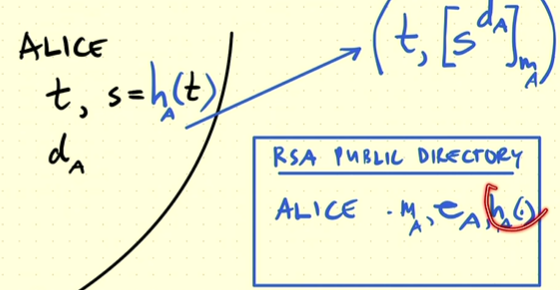
\includegraphics[scale=0.7]{22025-04-16.png}

\end{parag}
\begin{parag}{How does the public check?}
    \begin{subparag}{Step 1}
        \begin{equation*} \left[\left(\left[s^{d_A}\right]_m\right)^{e_a}\right]_m = s^a \end{equation*}
    \end{subparag}
    \begin{subparag}{Step 2}
        \begin{equation*} t \to h_A\left(t\right) = s \end{equation*}
        
    \end{subparag}
    \begin{subparag}{Step 3}
        if $s = $
        
    \end{subparag}
    
\end{parag}
\begin{parag}{Hash function}
    A hash function is a many-to one function, used to map a sequence of arbitrary length to a fixed length bit sequence of, say, 200 bits\\
    what we expect from a hash function, is that even the smallest change in the input produces a different output\\
    Ideally it should be so that one has to try about $2^{200}$ alternative inputs to hope to find a sequence that produces a given output.
    
\end{parag}


\begin{parag}{Digital Signature}
    to sign a document, we appends to the document a hash function of the docmunent in such  a way that only the signee could have done it 
    
\end{parag}


\begin{parag}{Trusted Agency}
    How do we know that the directory storing all the public keys has not been tampered with?
    \begin{subparag}{Example}
        Alies queries the public directory for bob's directory
        
    \end{subparag}
    \begin{subparag}{oui} 
        The directory information signed by a trusted agency, Say Symantex. Here is how:
       \begin{itemize}
           Symantec's public key is distributed one and for all via a channel that cannot be tapered with (e.g., hard coded into the crypto hardware)
           \item Each directory entry is digitally signed by symantec. We call the result a certificate
           \item Anybody that has Symantec's public key can verify that the information areceived from the directory is authentic
           
       \end{itemize}
       
       
   \end{subparag} 
\end{parag}
\subsection{Summary of chapter 2}
Perfect secrecy is possible but requires long keys:
\begin{parag}{One-time pad}
    In onte time pad, the cryptogram is compute like this:
    \begin{center}
        Cryptogram = Plaintext $ \oplus$ SharedKey
    \end{center}
    \begin{itemize}
        \item If the sharedKey is perfectly (uniformly) random and shared between encrypter and decrypter ahead of time
        \item and the sharedKey is kept secret from anyone else
        \item Then the One-time pad offers perfect secrecy
        \item Hence: it is expensive to implement. Only worth it for spies and such.
        
    \end{itemize}
\end{parag}
Practical cryptography is based on algorithmic/computational complexity\\
pPublic key cryptography. Most public key cryptographic algorithm fall into one of the following two categories:
\begin{itemize}
    \item those that are based on the belied that diescrete exponentiation (in mulitplicative cyclic group) is a one way function (e.g. Diffie-Hellamn and ElGamal)
    \item Those that are based on the difficulty of factoring (e.g. RSA)
\end{itemize}
To understand RSA and Diffie-Hellman, we need Number Theory and algebra.\subsection{Number theory and algebra}
First with modulo Operation and the euclid Algorithm (we can find the multiplicative inverse gcd etc\ldots.
\begin{parag}{Group}
    \begin{itemize}
        \item $ \mathbb{Z} / m \mathbb{Z}$ with addition is always a group
        \item $ \mathbb{Z} / m \mathbb{Z}$ with mulitplication: need to retain only those elements that have a multiplicative inverse: $ \mathbb{Z} / m \mathbb{Z}^*$
        \item Finding multiplicative inverses in $ \mathbb{Z} / m \mathbb{Z}$: Bézout identity; Extended Euclid algorithm
    \item How many element in $ \mathbb{Z} / m \mathbb{Z}$ have a multiplicative inverse? the answer is Euler's function (torient function) $\phi\left(n\right)$
    \item Group isomorphism
    \item Order of group elements Lagrance's theorem: Order of any group element must divide the cardinality of the group
    \end{itemize}
    
\end{parag}
\begin{parag}{Product group}
    \begin{theoreme}
    Main theorem: Cartesian product of groups is again a group
    \end{theoreme}
\end{parag}

\begin{parag}{The special Isomorphism}
    The special isomorphism between $ \mathbb{Z} / m_1m_2 \mathbb{Z}$ and $ \mathbb{Z} / m_1 \mathbb{Z} \times \mathbb{Z} / m_2 \mathbb{Z}$ when $m_1$ and $m_2$ are coprime:
    \begin{itemize}
        \item Holds for both addition and multiplication, including for elements that do not have multiplicative inverse,
        \item Hence, this is more than juste a group ismorphism
        
    \end{itemize}
    
    
\end{parag}


\subsubsection{Computationally hard problem}
\begin{parag}{Discrete logarithm}
    leads to Diffie Hellman( and, by slight extension, El Gamal)\\
    \begin{itemize}
        \item Encryption $A = g^a, B = g^b$
        \item Leads to a shered key: $C = A^b = B^a$
        \item To understand that it workds, we need cyclic groups.
    \end{itemize}
    
\end{parag}
\begin{parag}{Factorization of large integers}
    leads to Cocks and RSA.\\
    \begin{itemize}
        \item Encryption: $t^e \Mod m$ where $t$ is the plaintext and $m = pq$, where $p$ and $q$ are primes
        \item Decryption $\left(t^e\right)^d \Mod m$
        \item To understant that it works (meaning that $\left(t^e\right)^d \Mod m = t$ for all plaintexts t), we need to understand $ \mathbb{Z} / p \mathbb{Z} \times \mathbb{Z} / q \mathbb{Z}$
        
    \end{itemize}
    
    
\end{parag}
\begin{parag}{Authencity: Digital Signatures}
    In practice, so called symetric key cryptoSystems are important. The common secret key is typically only a few hundred bits, distributed e.g., via Diffie-Hellman. Encryption/decryption can be implemented more efficiently (faster  algorithm, smaller hardware). Think: one-time pad, but with an imperfect key. There is no proof that the resulting algorithm is secure.
    
\end{parag}





